
\documentclass[10pt,conference]{IEEEtran}
\usepackage{blindtext, graphicx}
\usepackage{listings}
\usepackage{listings}
\usepackage{subfig}
\usepackage{fancyhdr}
\usepackage{color}
\usepackage{graphicx}
\usepackage{amsmath}
\usepackage{amssymb}
\usepackage[english]{babel}
\usepackage[linesnumbered,boxed,commentsnumbered,ruled]{algorithm2e}
\usepackage{algorithmicx}
\usepackage{algpseudocode}
\usepackage{multirow}
\usepackage[sc]{mathpazo}
\usepackage[nocompress]{cite}
\renewcommand{\headrulewidth}{0pt}
\renewcommand{\footrulewidth}{0pt}
\newtheorem{Def1}{Definition}
\ifCLASSINFOpdf

\else

\fi



\hyphenation{op-tical net-works semi-conduc-tor}


\lstset{breaklines}

\lstset{extendedchars=false}
\lstset{
    language={[ANSI]C},
    morekeywords={co,all},
    frame=single,
    basicstyle=\small\ttfamily,
    keywordstyle=\small\ttfamily,
    % keywordstyle=\color{black}\bf,
    identifierstyle=,
    commentstyle=\usefont{T1}{pcr}{m}{sl}\color{black}\small,
    stringstyle=\color{black},
    breaklines,
    tabsize=2,
    captionpos=b
}


\begin{document}
%
% paper title
% can use linebreaks \\ within to get better formatting as desired
\title{A CPU-GPU Data Transfer Optimization Approach Based On Code Migration and Merging}
%
%
% author names and IEEE memberships
% note positions of commas and nonbreaking spaces ( ~ ) LaTeX will not break
% a structure at a ~ so this keeps an author's name from being broken across
% two lines.
% use \thanks{} to gain access to the first footnote area
% a separate \thanks must be used for each paragraph as LaTeX2e's \thanks
% was not built to handle multiple paragraphs
%

\author{
\IEEEauthorblockN{Cong Fu\IEEEauthorrefmark{1},  Yanlong Zhai\IEEEauthorrefmark{1},  Zhenhua Wang\IEEEauthorrefmark{2},
Muhammad Mudassar\IEEEauthorrefmark{1}, Zishuo Wang\IEEEauthorrefmark{1}}
\IEEEauthorblockA{\IEEEauthorrefmark{1}Beijing Engineering Research Center of Massive Language Information Processing and Cloud Computing Application\\ School of Computer Science, Beijing Institute of Technology, Beijing, China}
\{fucong, ylzhai\}@bit.edu.cn
\IEEEauthorblockA{\IEEEauthorrefmark{2}Beijing Institute of Control Engineering, Beijing, China}
zhenhuaw233@hotmail.com
}








\maketitle


% The paper headers

% The only time the second header will appear is for the odd numbered pages
% after the title page when using the twoside option.
%
% *** Note that you probably will NOT want to include the author's ***
% *** name in the headers of peer review papers.                   ***
% You can use \ifCLASSOPTIONpeerreview for conditional compilation here if
% you desire.




% If you want to put a publisher's ID mark on the page you can do it like
% this:
%\IEEEpubid{0000--0000/00\$00.00~\copyright~2007 IEEE}
% Remember, if you use this you must call \IEEEpubidadjcol in the second
% column for its text to clear the IEEEpubid mark.



% use for special paper notices
%\IEEEspecialpapernotice{(Invited Paper)}




% make the title area



\begin{abstract}
%\boldmath
Recent development in graphic processing units (GPUs) has subverted the traditional CPU-only computing. Because of the high performance and parallelism, GPUs are widely used as coprocessors to run highly parallel computations. However, porting applications to CPU-GPU architecture remains a challenge to average programmers, which have to explicitly manage data transfers between the host and device memories, and manually optimize GPU memory utilization. In this paper, we proposed an approach to optimize the data transfer operations between CPU and GPU by analysing the data dependency and reorganizing source code. Based on our previous work, we found that not only the data transmission through PCIe bus is time consuming, but also the preparation and cleaning work for data transfer operations. This cost will be dramatically increased if the program contains many kernel calls and sometimes the situation is getting severe when programmers are not sophisticated enough to make GPU programs. Therefore, we firstly defined and analyzed the data copy in (out) path for each data transfer operation utilizing compiler techniques. The data copy in or copy out operation can be migrated along with its data copy path. Multiple data transfer operations could be merged into one operation if they are of the same transfer direction and their data copy paths have overlap. Migrating and merging multiple data transfer operations could obviously reduce the number of data exchange times and the system resource consumption. The experimental results show that our approach has a significant effect on optimizing the parallel programs especially when the program has numerous kernel calls.

\end{abstract}
% IEEEtran.cls defaults to using nonbold math in the Abstract.
% This preserves the distinction between vectors and scalars. However,
% if the journal you are submitting to favors bold math in the abstract,
% then you can use LaTeX's standard command \boldmath at the very start
% of the abstract to achieve this. Many IEEE journals frown on math
% in the abstract anyway.

% Note that keywords are not normally used for peerreview papers.
\begin{IEEEkeywords}
GPU, data transfer, optimization, code migration, merging
\end{IEEEkeywords}






% For peer review papers, you can put extra information on the cover
% psage as needed:
% \ifCLASSOPTIONpeerreview
% \begin{center} \bfseries EDICS Category: 3-BBND \end{center}
% \fi
%
% For peerreview papers, this IEEEtran command inserts a pa2ge break and
% creates the second title. It will be ignored for other modes.
\IEEEpeerreviewmaketitle



\section{Introduction}
% \blindtext
Currently, even entry-level PCs are equipped with integrated Intel GPUs capable of hundreds of GFLOPS. Initially, GPUs were only used for graphics related computing, but due to their high processing power, now they are used as coprocessors to help CPU deal with high parallel and high computing operations. This helped a lot in performance gain and speed up the processes between 4x and 100x \cite{IEEEhowto:1}\cite{IEEEhowto:2}\cite{IEEEhowto:3}, but writing excellent parallel code is still a challenge for average programmers. For example, CUDA is a simple C-like interface proposed for programming NVIDIA GPUs, but it is difficult to port applications to CUDA which needs programmers to manage data transfer between the host and GPU memories explicitly \cite{IEEEhowto:4}. How to manage data transfer operations to optimize parallel programs is the focus of this paper.

In recent years, researchers around the world have adopted a number of ways to optimize parallel programs. Some optimizations are based on the GPU physical properties, such as vectorization (An array is represented as a vector and modify the code logic to use the correct element of the vector) \cite{IEEEhowto:5} to make full use of GPU cores, using read only data cache to store constants \cite{IEEEhowto:3}. Other optimization methods are based on common compiler optimization, such as loop invariant code motion (moving the invariant part out of loop structure) \cite{IEEEhowto:6}\cite{IEEEhowto:7} and loop unrolling (reducing or eliminating instructions that control the loop) \cite{IEEEhowto:8}. Table \ref{parallel_code_optimizations} shows some of the methods that have been applied to optimize parallel code.

\begin{table}[b]
  \centering
  \caption{parallel code optimizations}
  \begin{tabular}{ll}
    \hline
    % aftBackus:60er \\: \hline or \cline{col1-col2} \cline{col3-col4} ...
    Type                & Optimization      \\
    \hline
    Based on GPU      & Vectorization        \\
                      & Parallel loop swap   \\
                      & Texture fetching     \\
                      & Coalesced global memory access    \\
                      & Using read only data cache         \\
    General optimizations
                      & Loop unrolling     \\
                      &Common sub-expression elimination\\
                      &Loop invariant code motion\\
    \hline
  \end{tabular}
  \label{parallel_code_optimizations}
\end{table}

%We have done some research about big data computing on CPU-GPU cluster, and we have proposed some new design and optimization to speed up parallel programs with big data\cite{IEEEhowto:21}\cite{IEEEhowto:22}.
%Assume that above optimization methods have been done well enough, and GPU performance can be fully exploited now. Even so, we found that parallel programs were not as efficient as expected due to the typical CPU-GPU memory architecture.
The memory of CPU and GPU are isolated, so when the program switches between different processors, it is required to copy the data into the corresponding memory \cite{IEEEhowto:9}\cite{IEEEhowto:10}.
Data transfer between CPU and GPU is based on PCIe bus which bandwidth is about 16GB/s \cite{IEEEhowto:11}\cite{IEEEhowto:12}.
But the GPU memory bandwidth can be up to  100GB/s-250GB/s which is about 8 times of the CPU memory bandwidth. Therefore, the data transfer through PCIe bus must be the bottleneck of the system.
Due to the huge gap of the bandwidth, there will be a demonstrable delay when programmers can't manage data transfer reasonably on PCIe bus \cite{IEEEhowto:13}.
Our previous work designed a CPU/GPU collaboration framework based on Hadoop MapReduce to process the big data\cite{IEEEhowto:21}. We introduced a data flow analysis approach to optimize the data transfer between CPU and GPU\cite{IEEEhowto:22}. The approach can significantly improve the performance of the original program. But we also found that the performance is not only affected by the data transmission via PCIe, but also some system preparation work for opening and closing data transfer, especially in a parallel program with many kernels functions. Consumption of data transfer operations consists of transmission consumption on PCIe and system consumption for initializing and freeing. High frequency data transfer becomes the major factor of some inefficient programs. So optimizing this type of program becomes intensely important, particularly when programmers using some high level GPU grogram languages like OpenAcc, which may generate many kernel function calls.


 Using async data transfer can hide some cost, but it can not reduce actual cost of data transfer. This paper proposes a new approach to reduce system consumption for initializing and freeing by reducing the number of times of data transfer. We optimize the GPU source code by merging multiple data transfer operations after migrating them along the control flow based on compiler technique. Typically, a GPU kernel function call contains four steps: copy data into GPU memory, execute kernel function, copy result back to CPU memory, free data in GPU, and for most of time these four steps are called next to each other.
Data copy operations of different kernel functions do not have any overlap, which makes the program easy to understand, but some times it is not efficient enough.
In our work, we firstly analyse the data dependency of each data transfer operation, and define the data migration range for each of these operations. The data migration range is actually the positions in the source code where the data transfer operation can be moved to without changing the result of the program.
The migration range of different data transfer operations may have some overlaps which means multiple data transfer operations can be migrated to the same position.
After that, the best execution positions are calculated according to the algorithms defined by this paper with the aim of merging multiple data transfer operations into a single data transfer.
It is reasonable to make two transfer operations of different kernels executed at the same time if they are of the same transfer direction and the merging will not affect the result. By merging data transfer operations, we can reduce the number of times of data copy between CPU and GPU, even the total amount of data to transfer.


\section{migration of Data transfer operations }
Because of the different architecture, the CPU is good at performing sequential calculations, I/O, and program flow, and the GPU is
well suited for parallel data processing. Therefore, program runs on a  CPU/GPU environment always contains CPU code and GPU code.
CPU code usually has complex control logic and lower parallelism, GPU as a coprocessor has the ability to quickly perform complex mathematical and geometric calculations.
In the program flow, each kernel function requires two data transfers between CPU and GPU: the corresponding data need to be copied to GPU memory (hereafter referred to as the copyin) before kernel execution, and then copy the generated result back to CPU memory (hereafter referred to as the copyout) after the execution of kernel function. Afterwards, the data are freed(hereafter referred to as the data freeing) from GPU memory if it is not going to be used anymore.

\subsection{Migration constraints of data transfer operations}
A kernel execution process is divided into four separate phases: data copyin, execution, data copyout, and data freeing. Obviously, phases cannot be reversed, a kernel must be executed in the order of data copyin$\rightarrow$execution$\rightarrow$data copyout$\rightarrow$data freeing. But the time that each phase start to execute is adjustable. Data copyin operation can move forward alone the code control flow until the code line changes the data to be copied in. Data copyout operation can move backward along the code control flow to delay the data transfer, but it must be done before CPU code using the corresponding data. This is actually the data dependancy of the variables in the program. The data dependancy can be represented as the \textit{def-use chain} and \textit{use-def chain} and calculated by the compiler technique \emph{data flow analysis}.  After data copyout, GPU will perform data freeing operation immediately. But, if the data will be used in follow-up kernels again, we could make GPU keep holding the data until the follow-up kernels executed. This will reduce the total amount of data exchanges.

\subsection{Migration by code motion}
Now we will introduce how to adjust four phases described previously and how to migrate data transfer operations by code motion. As shown in listing \ref{Listing1}, the initial CUDA code structure describes that, data copyin, execution, data copyout, and data freeing operations are an integral whole. As shown in listing \ref{Listing2}, data copyin operation is executed in advance while data copyout and data freeing operations are postponed after migration. Apparently these migrations of data transfer operations do not affect result of the parallel program. Data copyin operation can move up along the code control flow, and it is legal to copy data to GPU memory before kernel execution and after the data changed in CPU code. Similarly data copyout operation can move down along the code control flow, and it is legal to copy out data to CPU memory after kernel execution and before the data used in CPU code. We call the conversion from the code structure in Listing 1 to the code structure in Listing 2 migration of data transfer operations.

\begin{lstlisting}[label=Listing1,caption=Initial CUDA code]
__global__ void kernel(int *device, int i);
int host[1000] = {0};
int tmp[1000] = {0};
for (int i = 0; i < 1000; i++)
    host[i] = host[i] + 1;
......
for (int i = 0; i < 1000; i++)
    tmp[i] = tmp[i]+1;
int *device;
CUDAMalloc(&device, sizeof(int) * 1000);
CUDAMemcpy(device, host, sizeof(int) * 1000, CUDAMemcpyHostToDevice); /*data copyin*/
for (int i = 0; i < 1000; i++) /*execution*/
    kernel<<<1,1>>>(device, i);
CUDAMemcpy(host, device, sizeof(int)* 1000, CUDAMemcpyDeviceToHost); /*data copyout*/
CUDAFree(device); /*data freeing*/
......
for (int i = 0; i < 1000; i++)
    tmp[i] = tmp[i]+1;
\end{lstlisting}

\begin{lstlisting}[label=Listing2,caption=After migration of data transfer operations]
__global__ void kernel(int *device, int i);
int host[1000] = {0};
int tmp[1000] = {0};
for (int i = 0; i < 1000; i++)
    host[i] = host[i]+1;
int *device;
CUDAMalloc(&device, sizeof(int) * 1000);
CUDAMemcpy(device, host, sizeof(int) * 1000, CUDAMemcpyHostToDevice); /*data copyin*/
......
for (int i = 0; i < 1000; i++)
    tmp[i] = tmp[i]+1;
for (int i = 0; i < 1000; i++) /*execution*/
    kernel<<<1,1>>>(device, i);
......
for (int i = 0; i < 1000; i++)
    tmp[i] = tmp[i]+1;
CUDAMemcpy(host, device, sizeof(int)* 1000, CUDAMemcpyDeviceToHost); /*data copyout*/
CUDAFree(device); /*data freeing*/
\end{lstlisting}

\section{Migrating algorithms}

\subsection{Basic block descriptions}

Because of the loop and conditional logic in the program, the source code are not executed sequentially, some parts of the code may be excluded  for execution. Therefore, the whole structure of the program need to be modelled for analyzing the possible migration ranges. In this paper, we leverage the concept of Basic Block (BB) from complier theory\cite{IEEEhowto:18}. In figure~\ref{figure1}(a), the code structure is divided into four BBs, a BB is a straight-line code control flow with no branches in except entry and no branches out except exit. A BB has only one entry point and only one exit point, so it must be entered from its entry and must be exited from exit\cite{IEEEhowto:20}. In figure \ref{figure1}(b), $BB_I$, $BB_J$, $BB_K$, $BB_L$ and control blocks branch (B), merger (M) make up the code structure described in figure \ref{figure1}(a). $BB_I$ is executed prior to $BB_L$, expressed as $BB_I < BB_L$. Each BB between $BB_I$ and $BB_L$ meets principle of $BB_I \le BB \le BB_L$. We have defined BBs which are in a pair of control blocks B and M as *BBs. $BB_K$ and $BB_J$ are *BBs in figure \ref{figure1}(b), with control blocks B, M making up a branch structure. $B_n$, $M_n$, and all *BBs which meet $B_n <$ *$BB$ $< M_n$ make up a branch structure $BRANCH_n$. Apparently not all *BBs will be executed, in figure \ref{figure1}b, within both $BB_K$ and $BB_J$, there's one and only one will be executed. If migrating a data transfer operation into a *BB, data exchange operation between CPU and GPU might not be executed, causing program to crash. The program does not know specific execution process in compile phase, unable to determine which *BB will be accessed. So each data exchange operation must be placed outside each branch in the code control flow to ensure implementation.






\begin{figure}
 \centering
 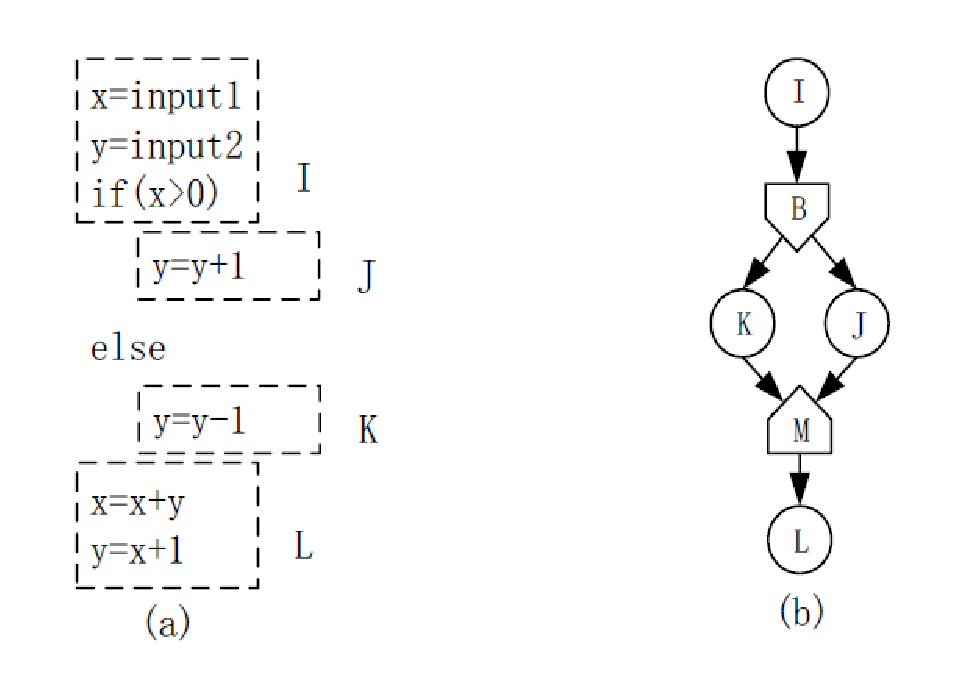
\includegraphics[width=3in]{image006.eps}
 \caption{Control Flow Graph}\label{figure1}
\end{figure}
\subsection{Migration algorithms for data transfer operations}
Entire program structure is composed of many code lines. Code at N-th line is expressed as $LINE_N$, and whole program structure is made up of [$LINE_1, LINE_{end}$]. Migration algorithms for data transfer operations are to obtain a largest set of code lines (copypath) to migrate data copyin or data copyout operations. This paper optimizes parallel programs from the perspective of data transfer, so we don't need to migrate kernel executions in parallel programs. Based on the BB, data copyin and data copyout operations are moved with code line unit. These algorithms are aimed at a single kernel, so we don't care whether the data after data copyout in GPU will be used again by subsequent kernels. After data copyout operation, GPU will free the data immediately in data freepath.



\subsubsection{Obtain data copyinpaths}
A data copyin operation can move upward along code control flow until current code line or current BRANCH changes (kills) the corresponding data. $LINE_i$ does not kill dataA expressed as  $\neg$$kill$(dataA, $LINE_i$), and each code line in $BRANCH_i$ does not kill dataA expressed as $\neg$$kill$(dataA, $BRANCH_i$). Algorithm \ref{alg:obtain_dataA_copypath} takes moving upward dataA copyin operation as an example, initial line of dataA copyin is lower bound of upward movement. Current BB is initial BB, and initial copyinpath is empty. If current BB is not *BB, moving dataA copyin operation upward along code control flow until code line would kill dataA or exit current BB. The line begins to move and line to exit make up a moving interval, then add the interval of code lines to copyinpath. If meeting exit point in current BB to exit, continue moving up and if killing dataA to exit, quit. When current BB is *BB, if all *BBs in current BRANCH do not kill dataA, moving up to exit current BRANCH and continue to generate copyinpath, otherwise quit. Final copyinpath is a largest set of code lines for moving dataA copyin operation.
\begin{Def1}
Given a dataA copyin operation at $LINE_n$, $\exists$$LINE_m$ with $\neg$$kill$(dataA, [$LINE_m, LINE_n$]) and $kill$(dataA, $LINE_{m-1}$), [$LINE_m, LINE_n$] $-$ codelines in BRANCHs is dataA copyinpath.
\end{Def1}

\subsubsection{Obtain data copyoutpath and freepath}
Data copyout operations can move down along code control flow until current code line or current BRANCH changes or gets value of the corresponding data ($use$ $data$). $LINE_i$ does not use dataA expressed as $\neg$$use$(dataA, $LINE_i$), and each code line in $BRANCH_i$ does not use dataA expressed as $\neg$$use$(dataA, $BRANCH_i$). Algorithm~\ref{alg:obtain_dataA_copyoutpath} describes how to obtain copyoutpath and freepath of dataA.
\begin{Def1}
Given a dataA copyout operation at $LINE_n$, $\exists$$LINE_m$ with $\neg$$use$(dataA, [$LINE_n, LINE_m$]) and $use$(dataA, $LINE_{m+1}$), [$LINE_n, LINE_m$] $-$ codelines in BRANCHs is dataA copyoutpath.
\end{Def1}

\begin{algorithm}
\KwIn{	copyinpath = $\emptyset$, $LINE_i$ = $LINE_j$ = initial line of dataA copyin operation}

\If{current BB is not *BB}{
     \While{$LINE_i$ in current BB  and $\neg$kill(dataA, $LINE_i$)}
        {$LINE_i$ = $LINE_i$ $-$ 1;}
     update current BB based on $LINE_i$;

     copyinpath = copyinpath +($LINE_i$, $LINE_j$];\

   \If {$kill$(dataA, $LINE_i$)}{
       end algorithm;
       }

}
   \uIf{$\neg$$kill$(dataA, current BRANCH)}{
       current BB = the BB before current BRANCH\;

       $LINE_i$ = $LINE_j$ = the last code line in current BB\;

       goto 1\;
       }
   \Else{
    end algorithm;}


\caption{Obtain dataA copyinpath}
\label{alg:obtain_dataA_copypath}
\end{algorithm}

\begin{algorithm}
\KwIn{	copyoutpath = $\emptyset$, $LINE_i$ = $LINE_j$ = initial line of dataA copyout operation}

\If{current BB is not *BB}{
     \While{$LINE_j$ in current BB  and $\neg$use(dataA, $LINE_j$) }
        {$LINE_j$ = $LINE_j$ + 1;}
     update current BB based on $LINE_j$;

     copyoutpath = copyoutpath +[$LINE_i$, $LINE_j$);\

     freepath = [$LINE_j$, $LINE_j$]\;

   \If {$use$(dataA, $LINE_j$)}{
       end algorithm;
       }

}

   \uIf{$\neg$$use$(dataA, current BRANCH)}{
       current BB = the BB after current BRANCH\;

       $LINE_i$ = $LINE_j$ = the first code line in current BB\;

       goto 1\;
       }
   \Else{
    end algorithm;}


\caption{Obtain dataA copyoutpath and freepath}
\label{alg:obtain_dataA_copyoutpath}
\end{algorithm}

\begin{figure*}
 \centering
 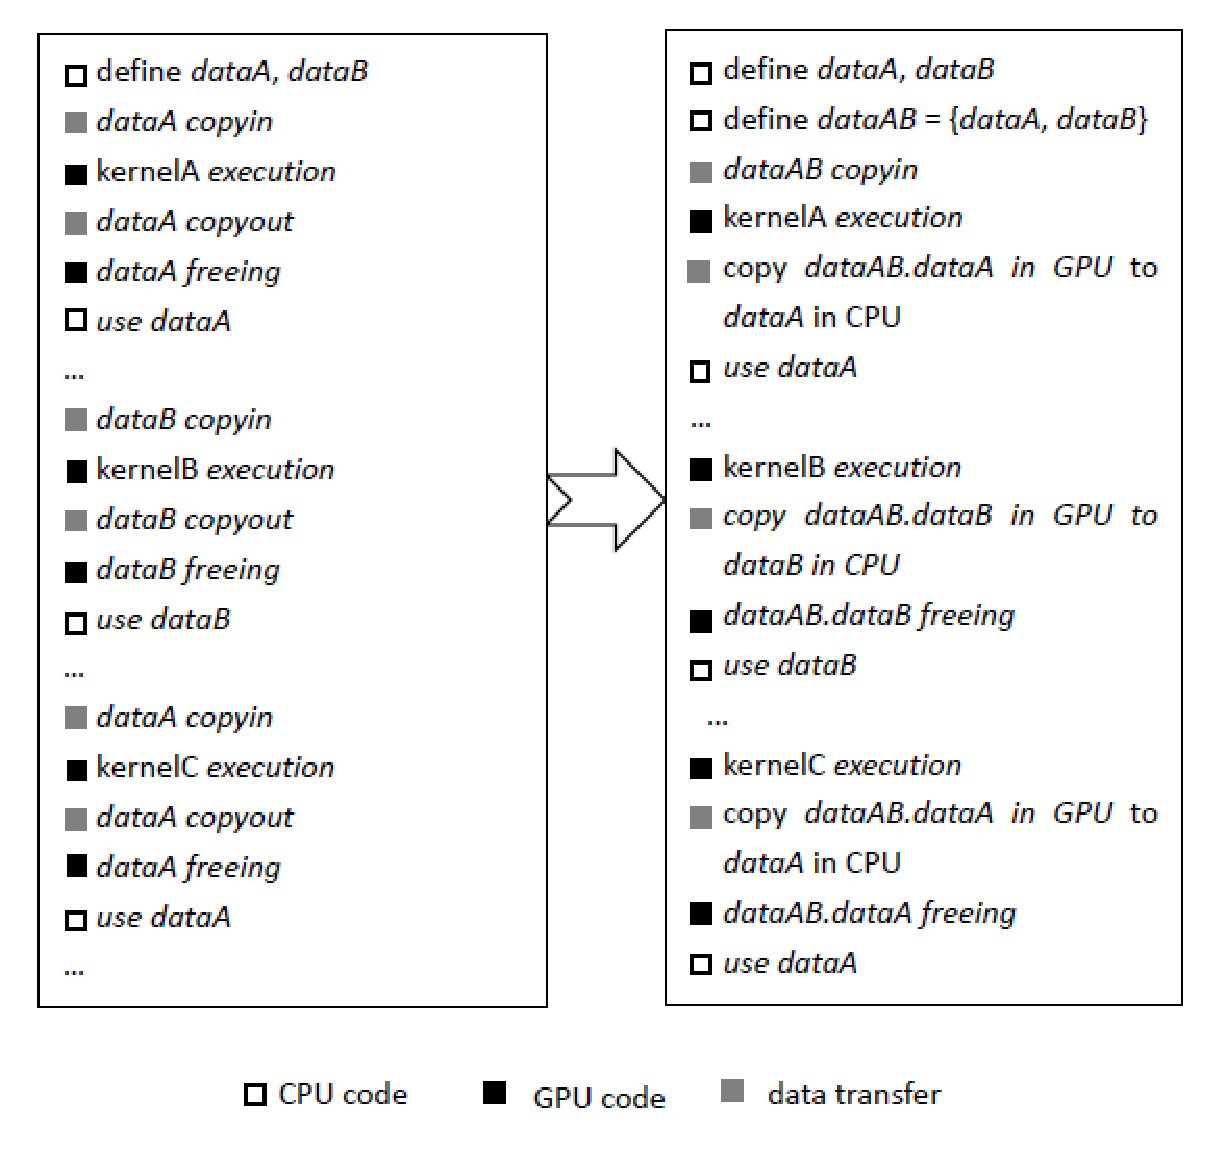
\includegraphics[width=5in]{image007.eps}
 \caption{Data transfer operations merging}\label{figure2}
\end{figure*}

\section{Merging of data transfer operations}
After migration, it is legal to make data copyin operations and data copyout operations executed at any code line in the corresponding copypaths. In a highly parallel program with multiple kernels, each kernel is no longer an independent entity, copyinpaths and copyoutpaths of different kernels will overlap. As shown in figure \ref{figure2} right, dataA copyinpath overlaps dataB copyinpath, merging two data copyin operations into one. Two things happened here, first we define a new data structure dataAB which size is size of dataA plus size of dataB in CPU memory, and copy dataA and dataB to dataAB. DataAB is a contiguous area of CPU memory, so we make dataAB copyin operation replaces dataA copyin and dataB copyin. Obviously, copying dataA and dataB to dataAB requires extra time and extra space in CPU memory. Assume that the memory space is sufficient, due to high CPU memory bandwidth (Intel Xeon Phi x200 processor, a single Haswell chip can deliver about 60 GB/s sustained memory bandwidth \cite{IEEEhowto:14}\cite{IEEEhowto:15}), extra time spent on CPU is very small. The total amount of data exchange does not reduce after merging, but the number of times to copy data to GPU operations decreased from two to one, reducing system consumption for opening and closing data transfer operations, making the best use of transmission bandwidth.In figure \ref{figure2} left, GPU frees dataA immediately after dataA copyout operation. CPU must copy dataA into GPU again before executing kernelC. Actually, dataA copyin operation of kernelC is not necessary, because this data is same as the data which kernelA frees. In figure \ref{figure2} right, dataA freeing operation of kernelA is cancelled and GPU memory will keep dataA, so kernerlC reuse dataA of kernelA and dataA copyin operation of kernelC is cancelled too. The total amount of data exchange is reduced after merging, hence speeded up program processing.

\subsection{Merging algorithms for data transfer operations}
Merging algorithms for data transfer operations consist of two part, one is merging data freepaths and copyin paths of different kernels to reduce the total amount of data exchange by data reuse, the other is merging data copyths to reduce the frequency of data transfer. Data copyinpaths, copyoutpaths and freepaths are obtained by Algorithm~\ref{alg:obtain_dataA_copypath} and Algorithm~\ref{alg:obtain_dataA_copyoutpath}, now we will describe how to merge data copypaths and freepaths of different kernels optimally.
\subsubsection{Merging data freepaths and copyinpaths}
GPU memory is not always enough, and it's useless for GPU to keep the data which will not be used in follow-up kernels. Based on four properties (data, copyinpath, copyoutpath, freepath) in each kernel, Algorithm~\ref{alg:delay_data_freeing} presents a smart solution.
\begin{Def1}
Given the kernels $K_i$ and $K_j$ with $K_i$.data==$K_j$.data and $K_i$.freepath $\cap$ K$_j$.copyinpath $\ne \emptyset$, the data freeing of $K_i$ and data copyin operation of $K_j$ can be cancelled, and $K_j$ will reuse the data of $K_i$.
\end{Def1}

\begin{algorithm}
    \ForEach{ kernel K$_i$ in kernel set}{

     \ForEach{ kernel K$_j$ in kernel set}{

            \If{ K$_i$.data == K$_j$.data and K$_i$.freepath $\cap$ K$_j$.copyinpath $\ne \emptyset$}{
                 K$_i$.freepath    = $\emptyset$;

                 K$_j$.copyinpath  = $\emptyset$;
                 }
        }
        }
\caption{Merge data freepaths and copyinpaths}
\label{alg:delay_data_freeing}
\end{algorithm}

\subsubsection{Merging data copypaths}
This algorithm will make each data transfer operation executed at a fixed code line in corresponding data copypath, then we will merge data copyin or copyout operations if they are at the same code line. Algorithm~\ref{alg:merge_copyinpaths} proposes a greedy strategy to merge data copypaths to minimize the number of times to copy data between CPU and GPU memories. Merging data copyoutpaths is the same as merging data copyinpaths, so we just describe how to merge copyinpaths. Initial kernel set contains all kernels. Define an array W, W[i] is the number of times LINE$_i$ is covered by all copyinpaths in current kernel set.
\begin{Def1}
Given the kernels $K_i$ and $K_j$ with $K_i$.copyinpath $\cap$ K$_j$.copyinpath $\ne \emptyset$, the data copyin operations of $K_i$ and $K_j$ can be merged into one data copyin operation.
\end{Def1}

\begin{algorithm}
   \While{kernel set is not empty}{

    W[1, end] = \{0\};\

    \ForEach{ kernel K$_i$ in kernel set}{

     \ForEach{ LINE$_j$ in K$_i$.copyinpath}
     {
        W[j] = W[j] + 1;
    }
   }

    n = W.findMaxIndex();

    \ForEach{ kernel K$_i$ in kernel set}
    {

    \If{LINE$_n$ in K$_i$.copyinpath}{

        K$_i$.copyinpath = [$LINE_n$, $LINE_n$];

         Remove K$_i$ from kernel set;
    }
    }
    goto 1;
}
\caption{Merge data copyinpaths}
\label{alg:merge_copyinpaths}
\end{algorithm}



\section{Evaluation}
Since our target is to optimize data transfer between CPU and GPU, we don't care what GPU code does and we can't reduce GPU execution time by the algorithms proposed in this paper. What we focus on is how to optimize parallel program by reducing the total amount and frequency of data exchange. So we take data transfer volume and data transfer frequency as experimental parameters, and take run-time of all data transfer operations which consist of all transmission consumption on PCIe and all system consumption for initializing and freeing as evaluating indicator.
\subsection{Experimental platform}
We use an Intel(R) Xeon(R) E5-2620 v2 @2.10GHZ CPU with 1.5MB of L2 cache to be the host CPU for the GPU. All GPU codes were executed on an ASPEED Graphics Family (rev 21) video card, a CUDA device with 4,799 MB of global memory. The CUDA driver version is release 5.5. The nvcc compiler release 5.5, V5.5.0 compiled all CUDA programs using default optimization level.
\begin{figure}
 \centering
 \includegraphics[width=0.9\linewidth]{image005.eps}
 \caption{Matrix size per kernel = 10 KB}\label{figure4}
\end{figure}
\begin{figure}
 \centering
 \includegraphics[width=0.9\linewidth]{image002.eps}
 \caption{Matrix size per kernel = 20 KB}\label{figure5}
\end{figure}
\begin{figure}
 \centering
 \includegraphics[width=0.9\linewidth]{image001.eps}
 \caption{Matrix size per kernel = 50 KB}\label{figure6}
\end{figure}


 \renewcommand\arraystretch{1.5}
 \begin{table*}[!htb]
  \centering
  \caption{Comparing parallel programs with and without merging data transfer operations}
  \begin{tabular}{|c|c|c|c|c|}
    \hline
    \multirow{2}{*}{amount of data transfer per kernel} &
    \multirow{2}{*}{number of kernels} &
    \multirow{2}{*}{without (us)} &
    \multicolumn{2}{|c|}{with(us)} \\
    \cline{4-5}
   & & & {copying operations in CPU} & {data transfer}\\
    \hline
    \multirow{4}{*}{1 KB}& 10 & 257 & 16 & 61\\
    \cline{2-5}
    & 50 & 1139 & 57 &102\\
     \cline{2-5}
     & 100 & 2378 & 141 &170\\
      \cline{2-5}
      & 500 & 11867 & 678 &633\\
      \hline
       \multirow{4}{*}{10 KB}& 10 & 345 & 122 & 153\\
    \cline{2-5}
    & 50 & 1844 & 586 &621\\
     \cline{2-5}
     & 100 & 3072 & 1085 &953\\
      \cline{2-5}
      & 500 & 18942 & 5699 &5020\\
      \hline
       \multirow{4}{*}{20 KB}& 10 & 566 & 231 & 281\\
    \cline{2-5}
    & 50 & 3003 & 1091 &943\\
     \cline{2-5}
     & 100 & 5260 & 2197 &1874\\
      \cline{2-5}
      & 500 & 26301 & 8835 &9835\\
      \hline
       \multirow{4}{*}{50 KB}& 10 & 768 & 552 & 526\\
    \cline{2-5}
    & 50 & 4007 & 2102 &2220\\
     \cline{2-5}
     & 100 & 10205 & 5574 &4989\\
      \cline{2-5}
      & 500 & 51428 & 21654 &22298\\
      \hline


  \end{tabular}
  \label{tab:pro_pro}
\end{table*}
\subsection{Experimental results}
Our experiments are performed with and without merging data transfer operations under a set of parallel programs for matrix addition with different matrix sizes and different numbers of kernels. In order to facilitate the experiment, in each parallel program, we let the matrix size per kernel is same and we make all data copyin operations and all data copyout operations can be merged into one data copyin operation and one data copyout operation. Figure \ref{figure4}, \ref{figure5} and \ref{figure6} show the data transfer time in microseconds for parallel programs without data transfer merging in comparison to with data transfer operations merging. The three histograms show the experimental results of parallel programs with different matrix sizes per kernel 10KB, 20KB, 50KB and different numbers of kernels 10, 50,100. The data transfer time of parallel program with data transfer operations merging is composed of the time to copy the data of different kernels to a new continuous CPU memory (yellow part in figure \ref{figure4}) and the time to transfer the continuous data to GPU memory (red part). From the experimental results we can see that the data transfer time of program with data transfer merging (red part) is obviously shorter than the data transfer time of program without data transfer merging (blue part). Because the red part contains little system consumption for initializing and closing data transfer operations. But when there is increase of the amount of data transferred per kernel, the proportion of the time spent copying operations in CPU memory (yellow part) is greater and greater, and even makes data transfer operations merging algorithm have side effect on parallel program. So, the algorithms proposed in this paper have significant optimization effect on data transfer of parallel programs when the data transfer volume is relatively small and data exchange is frequent. Table \ref{tab:pro_pro} shows more experimental results.




\section{Related Work}
Although there has been prior work on optimizing parallel computing for CPU-GPU architecture, these implementations have not addressed how to migrate and merge data transfer operations of different kernels between CPU and GPU memories. Many scholars, according to the memory structure and multi-core characteristic of GPU have proposed some optimization methods to optimize parallel computing on CPU-GPU architecture.

First we can optimize parallel programs to make full use of GPU computing resources and GPU memory resources through manual code analysis and modifications. Vectorization can be applied by using vector data types provided in CUDA as data structure and modify the code logic to use the correct element of the vector in other expressions \cite{IEEEhowto:4}\cite{IEEEhowto:16}. Vectorization can make full use of multi-core characteristic of GPU and open more threads to run parallel computing. Texture memory can be used in kernels by invoking texture intrinsic provided in CUDA\cite{IEEEhowto:19}. It needs to be bound explicitly to CUDA array allocated in device memory. Rational use of texture memory can significantly optimize parallel programs.

Then, there are some optimizations on parallel programs in the compilation phase. Loop Collapsing is performed by merging double or more nested loops into a single loop which can be done by loop analysis and transformation within the compiler \cite{IEEEhowto:4}\cite{IEEEhowto:17}. Loop Collapsing can increase the degree of parallelism compared with initial nested loops, and GPU will open more threads to run the loop. Thread and Thread-Block Merging can be achieved by duplicating the global memory array expressions identified by the programmer with incrementing the array indices and modifying the main loop partitioning based on the thread granularity defined by the programmer \cite{IEEEhowto:4}. And using read only data cache to store constants in GPU can speedup GPU memory access \cite{IEEEhowto:3}. And researchers found that optimizing programs by analyzing the structure of source code and reorganizing source code has a significant optimization effect. For example, at any point in time of program process, the program can't make full use of all system computing resources\cite{IEEEhowto:20}. Because computing resources have some different types, program generally takes up one at a code line in program. Some researchers have proposed a smart algorithm that compiler migrates the subsequent code to current point legally to use free computing resourse. Data dependency and program logic are the most important criterions of code migration for programmers. A reasonably strategy of code migration can speed up program process by making program take up more system computing resources.
\section{Conclusion}
We propose a new method to optimize parallel computing on CPU-GPU architecture by just optimizing data transfer between CPU and GPU memories. We don't reduce the transmission consumption on PCIe, but we reduce the system consumption for initializing and freeing by reducing the number of times of data transfer. Our algorithms consist of two parts, one is migrating each data transfer operation by code motion in parallel program, and the other is merging data transfer operations of different kernels with greedy strategy after migrating. Through a series of experimental results, our algorithms have been proved to have a significant optimization effect on parallel computing when the data transfer volume is relatively small and data exchange is frequent. In a parallel program which has more than 10 kernels and the average amount of data transfer each kernel less than 20KB, we can reduce the total data transfer time by about 20\% by the algorithms proposed in this paper.




% if have a single appendix:
%\appendix[Proof of the Zonklar Equations]
% or
%\appendix  % for no appendix heading
% do not use \section anymore after \appendix, only \section*
% is possibly needed

% use appendices with more than one appendix
% then use \section to start each appendix
% you must declare a \section before using any
% \subsection or using \label (\appendices by itself
% starts a section numbered zero.)
%


%\appendices
%\section{Proof of the First Zonklar Equation}
%Some text for the appendix.

% use section* for acknowledgement


\section*{Acknowledgment}
 We thank the entire Beijing Institute of Control Engineering for their support and feedback during this work. We also thank Wenjun Tao for generously proposing their useful amendments and addendum to this paper. Additionally, We thank the anonymous reviewers for their insightful comments.

 This work is supported by NSFC (National Natural Science Foundation of China) grants 61602037.
% Can use something like this to put references on a page
% by themselves when using endfloat and the captionsoff option.
%\ifCLASSOPTIONcaptionsoff
 %
%\fi



% trigger a \newpa just before the given reference
% number - used to balance the columns on the last page
% adjust value as needed - may need to be readjusted if
% the document is modified later
%\IEEEtriggeratref{8}
% The "triggered" command can be changed if desired:
%\IEEEtriggercmd{\enlargethispage{-5in}}

% references section

% can use a bibliography generated by BibTeX as a .bbl file
% BibTeX documentation can be easily obtained at:
% http://www.ctan.org/tex-archive/biblio/bibtex/contrib/doc/
% The IEEEtran BibTeX style support page is at:
% http://www.michaelshell.org/tex/ieeetran/bibtex/
%\bibliographystyle{IEEEtran}
% argument is your BibTeX string definitions and bibliography database(s)
%\bibliography{IEEEabrv,../bib/paper}
%
% <OR> manually copy in the resultant .bbl file
% set second argument of \begin to the number of references
% (used to reserve space for the reference number labels box)

\begin{thebibliography}{1}

\bibitem{IEEEhowto:1}
D.~M.~Dang, C.~Christara, and K.~Jackson, \emph{GPU pricing of exotic cross-currency interest rate derivatives with a foreign exchange olatility skew model.}\hskip 1em plus 0.5em minus 0.4em\relax SSRN eLibrary, 2010.
\bibitem{IEEEhowto:2}
D.~R. Horn, M.~Houston, and P.~Hanrahan, \emph{A streaming hmmer-search implementation.}\hskip 1em plus 0.5em minus 0.4em\relax Proceedings of the Conference on supercomputing (SC), 2005.
\bibitem{IEEEhowto:3}
S.~Ryoo, C.~I. Rodrigues, S.~S. Baghsorkhi, S.~S. Stone, D.~B. Kirk, and W.~Hwu, \emph{Optimization principles and application performance evaluation of a multithreaded GPU using CUDA.}\hskip 1em plus 0.5em minus 0.4em\relax In proceedings of the Thirteenth ACM SIGPLAN Symposium on Principles and Practice of Parallel Programming (PPoPP), 2008.
\bibitem{IEEEhowto:4}
AH Khan, M Al-Mouhamed, M Al-Mulhem, and Adel F. Ahmed, \emph{RT-CUDA: A Software Tool for CUDA Code Restructuring.}\hskip 1em plus 0.5em minus 0.4em\relax International Journal of Parallel Programming, 2016.
\bibitem{IEEEhowto:5}
A Kawai, K Yasuoka, K Yoshikawa, and T Narumi, \emph{Distributed-shared CUDA: Virtualization of large-scale GPU systems for programmability and reliability.}\hskip 1em plus 0.5em minus 0.4em\relax The Fourth International Conference on Future Computational Technologies and Applications (FUTURE COMPUTING), 2012.
\bibitem{IEEEhowto:6}
P Colea, F Luporini, and PHJ Kelly, \emph{Generalizing loop-invariant code motion in a real-world compiler.}\hskip 1em plus 0.5em minus 0.4em\relax MEng Computing Individual Project, 2015.
\bibitem{IEEEhowto:7}
Diogo Sampaio, Alain Ketterlin, Louis-Noel Pouchet, and Fabrice Rastello, \emph{Hybrid data dependence analysis for loop transformations.}\hskip 1em plus 0.5em minus 0.4em\relax Parallel Architecture and Compilation Techniques (PACT), 2016.
\bibitem{IEEEhowto:8}
Manato Hirabayashi, Shinpei Kato, and Masato Edahiro, \emph{Accelerated Deformable Part Models on GPUs.}\hskip 1em plus 0.5em minus 0.4em\relax IEEE Transactions on Parallel and Distributed Systems , 2016.
\bibitem{IEEEhowto:21}
Yanlong Zhai, Emmanuel Mbarushimana, Wei Li, Jing Zhang, and Ying Guo, \emph{Lit: A High Performance Massive Data Computing}.\hskip 1em plus 0.5em minus 0.4em\relax international conference on cluster computing, 2013
\bibitem{IEEEhowto:22}
Yanlong Zhai, Ying Guo, Qiurui Chen, Kai Yang and Emmanuel Mbarushimana, \emph{Design and Optimization of a Big Data Computing Framework based on CPU/GPU Cluster}.\hskip 1em plus 0.5em minus 0.4em\relax IEEE International Conference on High Performance Computing and Communications,2013
\bibitem{IEEEhowto:9}
B.~Van Werkhoven, J.~Maassen, F.~J. Seinstra, \emph{Performance Models for CPU-GPU Data Transfers.}\hskip 1em plus 0.5em minus 0.4em\relax Cluster, Cloud and Grid Computing (CCGrid), 2014.
\bibitem{IEEEhowto:10}
Janghaeng Lee, Mehrzad Samadi, and Yongjun Park, \emph{Transparent CPU-GPU collaboration for data-parallel kernels on heterogeneous systems.}\hskip 1em plus 0.5em minus 0.4em\relax Parallel Architectures and Compilation Techniques (PACT), 2013.
\bibitem{IEEEhowto:11}
Fernando Martinez Vallina and Spenser Gilliland, \emph{Performance optimization for a SHA-1 cryptographic workload expressed in OpenCL for FPGA execution.}\hskip 1em plus 0.5em minus 0.4em\relax IWOCL '15 Proceedings of the 3rd International Workshop on OpenCL, 2015.
\bibitem{IEEEhowto:12}
D.~Cesini, A.~Ferraro, and A.~Falabella, \emph{High throughput data acquisition with InfiniBand on x86 low-power architectures for the LHCb upgrade.}\hskip 1em plus 0.5em minus 0.4em\relax Real Time Conference (RT), 2016.
\bibitem{IEEEhowto:13}
Akira Nukada, Yasuhiko Ogata, Toshio Endo, and Satoshi Matsuoka, \emph{Bandwidth intensive 3-D FFT kernel for GPUs using CUDA.}\hskip 1em plus 0.5em minus 0.4em\relax Proceedings of ACM/IEEE conference on Supercomputing, 2008.
\bibitem{IEEEhowto:14}
Jason Howard, Saurabh Dighe, and Yatin Hoskote, \emph{A 48-Core IA-32 message-passing processor with DVFS in 45nm CMOS.} \hskip 1em plus 0.5em minus 0.4em\relax Solid-State Circuits Conference Digest of Technical Papers (ISSCC), 2010.
\bibitem{IEEEhowto:15}
A.~Jain, W.~Anderson, and T.~Benninghoff, \emph{A 1.2 GHz Alpha microprocessor with 44.8 GB/s chip pin bandwidth.} \hskip 1em plus 0.5em minus 0.4em\relax Solid-State Circuits Conference, 2001.
\bibitem{IEEEhowto:16}
David F Bacon, Susan L Graham, and Oliver Sharp, \emph{Compiler transformations for high-performance computing.}\hskip 1em plus 0.5em minus 0.4em\relax ACM Computing Surveys, 1944.
\bibitem{IEEEhowto:17}
Mikhail Plotnikov, Andrey Naraikin, and Elmoustapha Ouldahmedvall, \emph{Collapsing of multiple nested loops, methods and instructions.}
\bibitem{IEEEhowto:18}
Ying Chen, \emph{Fundamentals of Compiling.}\hskip 1em plus 0.5em minus 0.4em\relax Beijing Institute of Technology press, 2001.
\bibitem{IEEEhowto:19}
J M Schneider and Rudiger Westermann, \emph{Compression domain volume rendering}.\hskip 1em plus 0.5em minus 0.4em\relax ieee visualization, 2003.
\bibitem{IEEEhowto:20}
Luiz C. V. dos Santos and Jochen A. G. Jess, \emph{A Reordering Technique for Efficient Code Motion}.\hskip 1em plus 0.5em minus 0.4em\relax ACM, 1999.
\end{thebibliography}

% biography section
%
% If you have an EPS/PDF photo (graphicx package needed) extra braces are
% needed around the contents of the optional argument to biography to prevent
% the LaTeX parser from getting confused when it sees the complicated
% \includegraphics command within an optional argument. (You could create
% your own custom macro containing the \includegraphics command to make things
% simpler here.)
%\begin{biography}[{\includegraphics[width=1in,height=1.25in,clip,keepaspectratio]{mshell}}]{Michael Shell}
% or if you just want to reserve a space for a photo:

\begin{IEEEbiography}[{\includegraphics[width=1in,height=1.25in,clip,keepaspectratio]{picture}}]{John Doe}
\blindtext
\end{IEEEbiography}

% You can push biographies down or up by placing
% a \vfill before or after them. The appropriate
% use of \vfill depends on what kind of text is
% on the last page and whether or not the columns
% are being equalized.

%\vfill

% Can be used to pull up biographies so that the bottom of the last one
% is flush with the other column.
%\enlargethispage{-5in}



% that's all folks
\end{document}

